\chapter{HỆ THỐNG EASYMESH}
\label{chapter:chapter-2}
\section{Tổng quan hệ thống Wi-Fi Mesh}
Một hệ thống Wi-Fi Mesh bao gồm những điểm truy cập không dây (Access Point - AP) với mục đích mở rộng vùng phủ sóng của Wi-Fi lên không gian vật lý, để tăng số lượng thiết bị kết nối (Station - STA) và sử dụng được dịch vụ Wi-Fi trong một không gian lớn hơn mà chỉ cần một cấu hình Wi-Fi được đồng bộ cho tất cả các AP. Các thành phần trong một mạng Wi-Fi Mesh được mô tả như hình \ref{fig:EasyMeshSystemModel} dưới đây, bao gồm các thành phần sau:

\begin{enumerate}
\item Controller: Một AP được thiết lập với vai trò Controller, làm nhiệm vụ là điểm ra kết nối mạng Internet cho toàn mạng mesh, là điểm kết nối tới của các Agent và các STA trong mạng, các cấu hình Wi-Fi thiết lập cho mạng Mesh được cấu hình duy nhất trên thiết bị này và sẽ được đồng bộ tới các Agent trong mạng.
\item Agent: Một AP được thiết lập với vai trò Agent, làm nhiệm vụ kết nối tới Controller và điểm truy cập không dây và có dây cho các STA. Nó nhận cấu hình từ Controller theo chuẩn IEEE 1905.1 và áp dụng cấu hình này xuống chính các Agent này.
\item AlMac: Một địa chỉ định danh cho các thiết bị trong mạng Mesh theo chuẩn IEEE 1905.1, nó như là tên của các thiết bị trong mạng mesh, và các bản tin 1905 được sử dụng AlMac này làm địa chỉ đích và địa chỉ nguồn. Đối với các bản tin MultiCast thì đại chỉ đích sẽ là 01:80:C2:00:00:13 theo chuẩn.
\item fBSS: Fronthaul BSS, một kết nối Wi-Fi trên Agent tới Controller.
\item bBSS: Backhaul BSS, một vùng phủ Wi-Fi phát từ Controller cho Agent kết nối đến BSS này.
\item bSTA: Backhaul STA, một vùng phủ Wi-Fi phát từ AP cho các STA kết nối tới BSS này.
\end{enumerate}

\begin{figure}
\centering
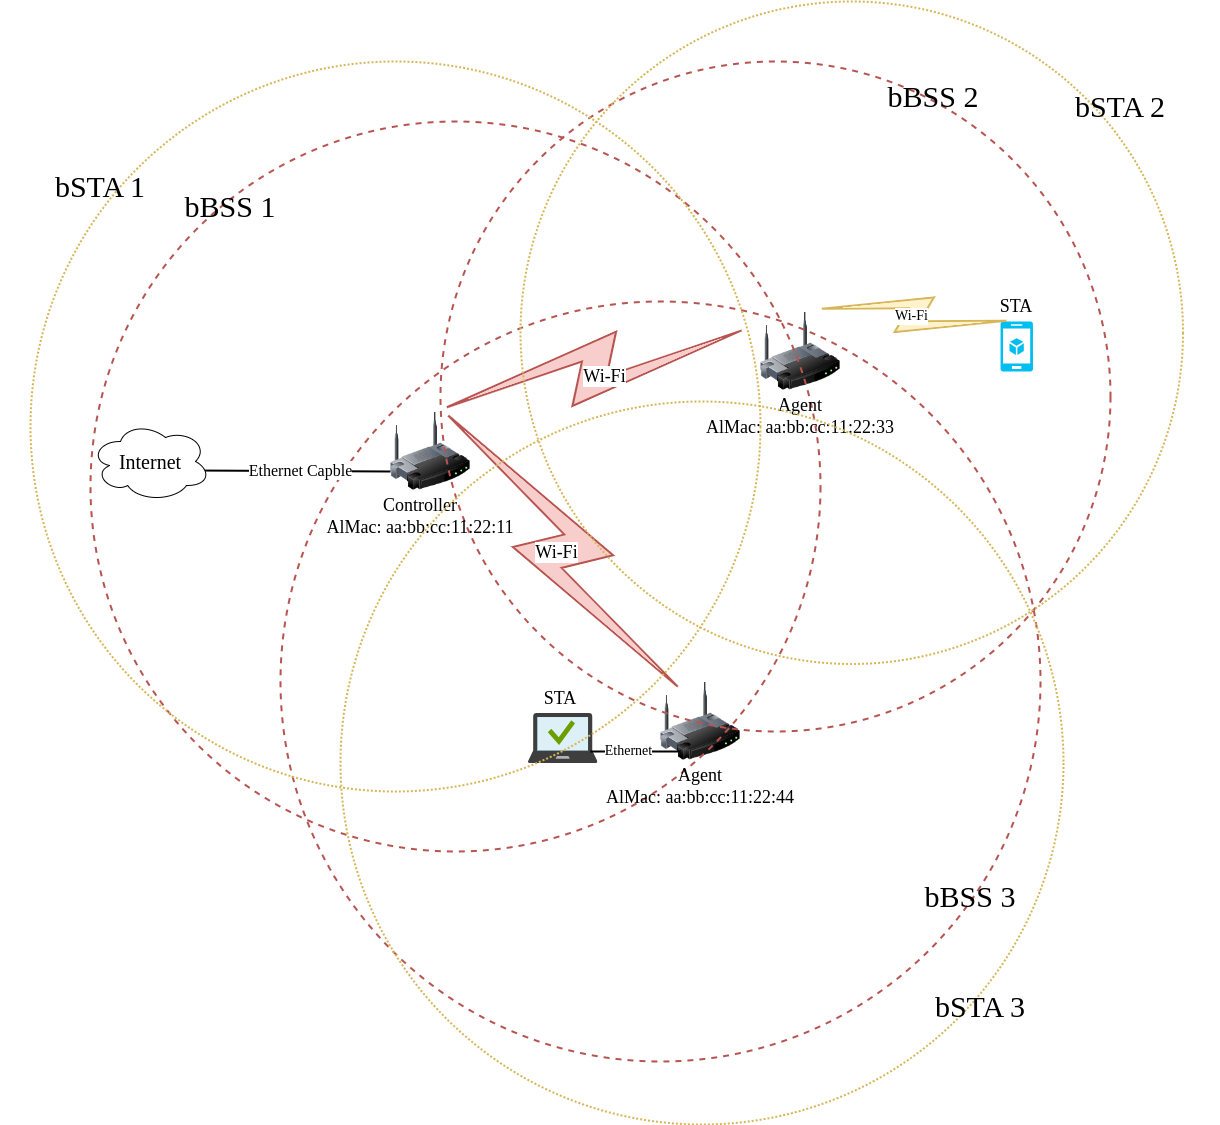
\includegraphics[width=1\textwidth]{mainmatter/images/EasyMeshSystemModel.png}
\caption{\label{fig:EasyMeshSystemModel}Mô hình một mạng Wi-Fi mesh.}
\end{figure}

Trên hình \ref{fig:EasyMeshSystemModel}, các bSTA được biểu diễn là hình tròn có viền là nét đứt màu vàng, bBSS được biểu diễn là hình tròn có viền là nét đứt màu hồng. Các liên kết giữ fBSS của Agent tới bBSS của Controller là kết nối Wi-Fi màu hồng, các kết nối Wi-Fi của các STA tới bBSS trên AP tô màu vàng.

\subsection{Triển khai thực tế hệ thống Wi-Fi Mesh của VHT}
Tính từ thời điểm 12/2024 hệ thống Wi-Fi Mesh của VHT đã được triển khai trên 64 tỉnh của Việt Nam, với hai dòng thiết bị của ONT và AP sử dụng Wi-Fi 5 và Wi-Fi 6. Thực tế các thiết bị này được mesh không chỉ cùng thế hệ Wi-Fi mà thậm chỉ cả chéo giữa các dòng Wi-Fi này. Dưới đây là một số trường hợp triển khai hệ thống dưới thị trường.

\begin{enumerate}
    \item ONTw5 - APw5
    \item ONTw5 - APw6
    \item ONTw6 - APw6
\end{enumerate}

Hiện tại, có thể triển khai thực tế 6 mô hình triển khai trên với thứ tự lần lượt gồm một Controller và nhiều Agent như liệt kê trên. Thực hiện mesh giữa các thiết bị cùng thế hệ Wi-Fi sẽ thoải mái hơn việc mesh giữa các thiết bị khác thế hệ Wi-Fi. Bởi lẽ, thông số liên quan đến Wi-Fi của 5 và 6 có những điểm khác biệt liên quan đến tốc độ kết nối vật lý, băng thông dẫn đến ảnh hưởng đến các thông số tính toán của hệ thống. Đây là điểm cần chú ý để tránh các lỗi xảy ra khi mesh giữa chúng.

\section{Các chức năng của hệ thống Wi-Fi Mesh}
\subsection{Đồng bộ cấu hình}

Chức năng đầu tiên mà một hệ thống Wi-Fi Mesh cần đáp ứng, việc này thực hiện việc đồng bộ các cấu hình từ Controller xuống tất cả các Agent được quản lý trong mạng. Quá trình này sẽ bắt đầu từ bước kết nối vật lý giữa Controller và Agent bằng hai cách là kết nối Wi-Fi hoặc kết nối có dây Ethernet. Sau khi kết nối thành công, các bản tin đồng bộ theo chuẩn IEEE 1905.1 sẽ được gửi đi và các Agent sẽ nhận và tách thông tin cấu hình từ bản tin này để cấu hình xuống Driver Wi-Fi. Thứ tự các bản tin được thể hiện như hình \ref{fig:Autoconfig}, và vai trò của các bản tin này sẽ được trình bày tóm tắt dưới đây:

\begin{figure}[ht]
\centering
\begin{tikzpicture}[
    node distance=4cm,
    >=Stealth,
    font=\small,
    device/.style={align=center},
    line/.style={-Latex, thick},
]

% Nodes
\node[device] (NewDevice) at (0,0) {New Device\\(Unconfigured)};
\node[device] (Controller) at (6,0) {Controller\\(Configured Device)};

% Lifelines
\draw[dashed] (NewDevice) -- ++(0,-4);
\draw[dashed] (Controller) -- ++(0,-4);

% Arrows
\draw[line] (NewDevice.south) ++(0,-1) -- ++(6,0) node[midway, above] {Autoconfig Search};

\draw[line] (Controller.south) ++(0,-2) -- ++(-6,0) node[midway, below] {Autoconfig Response};

\end{tikzpicture}
\caption{Luồng bản tin Autoconfig Search và Autoconfig Response trong IEEE 1905.1}
\label{fig:autoconfig-flow}
\end{figure}

\begin{figure}[ht]
\centering
\begin{tikzpicture}[
    node distance=2cm,
    >=Stealth,
    font=\small,
    device/.style={align=center},
    line/.style={-Latex, thick},
]

% Nodes
\node[device] (Enrollee) at (0,0) {Enrollee\\(Agent)};
\node[device] (Registrar) at (6,0) {Registrar\\(Controller)};

% Lifelines
\draw[dashed] (Enrollee) -- ++(0,-4.5);
\draw[dashed] (Registrar) -- ++(0,-4.5);

% Arrows
\draw[line] (Enrollee.south) ++(0,-1) -- ++(6,0) node[midway, above] {M1: Public Key, Nonce, Device Info};

\draw[line] (Registrar.south) ++(0,-2.5) -- ++(-6,0) node[midway, below] {M2: Public Key, Encrypted Settings (SSID, PSK)};

\end{tikzpicture}
\caption{Luồng bản tin M1/M2 trong quá trình bắt tay bảo mật (WPS hoặc Secure Link Setup)}
\label{fig:m1-m2-flow}
\end{figure}

\begin{enumerate}
\item Autoconfig Search: Bản tin này được gửi từ Agent với địa chỉ đích là một địa chỉ MultiCast theo chuẩn, bản tin này được chuyển tiếp tại Agent còn lại và phản hồi bởi duy nhất Controller. Trong trường hợp không nhận được phản hồi từ Controller sau thời gian trễ nhất định, Agent sẽ tiếp tục gửi lại bản tin này và tùy theo thiết kế phần mềm, số lần gửi và thời gian đợi cũng sẽ khác nhau.
\item Autoconfig Response: Bản tin này được gửi từ Controller khi Controller nhận được Autoconfig Search từ Agent. Bản tin này sẽ chứa thông tin của Controller giúp Agent thực hiện bước tiếp theo trong quá trình đồng bộ. Hai bản tin này sẽ có Message ID giúp xác nhận từng cặp bản tin, nếu nhận được bản tin khác ID này thì bản tin sẽ bị loại bỏ.
\item Autoconfig M1: Bản tin này được gửi từ Agent khi Agent nhận được bản tin Autoconfig Response từ Controller, nội dung bản tin này chứa những thông tin liên quan đến cấu hình có thể cài đặt về mạng Wi-Fi của Agent, giúp Controller lựa chọn và gửi đi cấu hình phù hợp nhất với khả năng của Agent. 
\item Autoconfig M2: Bản tin này được gửi từ Controller tới Agent chứa thông tin cấu hình Wi-Fi của Controller muốn Agent cập nhật. Các thông tin này bao gồm tên SSID, mật khẩu, kiểu mã hóa, thông tin của BSS tương ứng. Thông thường với các hệ thống mạng Mesh 2 băng tần 2.4GHz và 5GHz ta sẽ có 2 cặp bản tin M1-M2 tương ứng với cấu hình cho 2 băng tần kể trên.
\end{enumerate}

\begin{table}[ht]
\centering
\caption{Nội dung bản tin M1 trong WPS (Wi-Fi Protected Setup)}
\begin{tabular}{|>{\raggedright\arraybackslash}m{4cm}|>{\raggedright\arraybackslash}m{9cm}|}
\hline
\textbf{Trường (Field)} & \textbf{Mô tả} \\
\hline
Version & Phiên bản WPS, thường là 0x10 (WPS v1.0) \\
\hline
Message Type & Mã xác định bản tin là M1 (value = 0x04) \\
\hline
Registrar Nonce & Số nonce do thiết bị Registrar (Controller) tạo ra, dùng để tránh replay attack \\
\hline
UUID-E & UUID của thiết bị Enrollee (Agent) để nhận dạng duy nhất \\
\hline
Public Key & Khóa công khai (Public Key) của thiết bị Enrollee dùng cho trao đổi khóa Diffie-Hellman \\
\hline
Authentication Type Flags & Các loại phương pháp xác thực mà Enrollee hỗ trợ (ví dụ: WPA2-PSK) \\
\hline
Encryption Type Flags & Các loại mã hóa mà Enrollee hỗ trợ (ví dụ: AES) \\
\hline
Connection Type Flags & Thông tin loại kết nối (như băng tần 2.4GHz hoặc 5GHz) \\
\hline
Configuration Methods & Các phương pháp cấu hình hỗ trợ (như Push Button, PIN) \\
\hline
Manufacturer & Tên nhà sản xuất thiết bị Enrollee \\
\hline
Model Name & Tên mẫu thiết bị Enrollee \\
\hline
Model Number & Số hiệu mẫu thiết bị Enrollee \\
\hline
Serial Number & Số serial thiết bị Enrollee \\
\hline
Primary Device Type & Loại thiết bị chính (ví dụ: Access Point) \\
\hline
Device Name & Tên thiết bị Enrollee (có thể hiển thị trong UI) \\
\hline
\end{tabular}
\end{table}

\begin{table}[ht]
\centering
\caption{Nội dung bản tin M2 trong WPS (Wi-Fi Protected Setup)}
\begin{tabular}{|>{\raggedright\arraybackslash}m{4cm}|>{\raggedright\arraybackslash}m{9cm}|}
\hline
\textbf{Trường (Field)} & \textbf{Mô tả} \\
\hline
Version & Phiên bản WPS, thường là 0x10 (WPS v1.0) \\
\hline
Message Type & Mã xác định bản tin là M2 (value = 0x05) \\
\hline
Enrollee Nonce & Số nonce do thiết bị Enrollee tạo ra (từ bản tin M1) \\
\hline
Public Key & Khóa công khai của Registrar (Controller) dùng cho trao đổi khóa Diffie-Hellman \\
\hline
Authentication Type Flags & Các loại phương pháp xác thực mà Registrar hỗ trợ (ví dụ: WPA2-PSK) \\
\hline
Encryption Type Flags & Các loại mã hóa mà Registrar hỗ trợ (ví dụ: AES) \\
\hline
Connection Type Flags & Thông tin loại kết nối (như băng tần 2.4GHz hoặc 5GHz) \\
\hline
Configuration Methods & Các phương pháp cấu hình hỗ trợ (như Push Button, PIN) \\
\hline
Manufacturer & Tên nhà sản xuất thiết bị Registrar \\
\hline
Model Name & Tên mẫu thiết bị Registrar \\
\hline
Model Number & Số hiệu mẫu thiết bị Registrar \\
\hline
Serial Number & Số serial thiết bị Registrar \\
\hline
Primary Device Type & Loại thiết bị chính (ví dụ: Access Point) \\
\hline
Device Name & Tên thiết bị Registrar (có thể hiển thị trong UI) \\
\hline
Encrypted Settings & Dữ liệu mã hóa chứa SSID, mật khẩu (PSK) và các cấu hình Wi-Fi khác \\
\hline
\end{tabular}
\end{table}

\subsection{Quản lý thiết bị}
Việc quản lý các thiết bị trong mạng Mesh được thực hiện dựa trên giao tiếp bản tin theo chuẩn IEEE 1905.1 giữa các thiết bị trong mạng và thường được quản lý tập trung tại Controller. Những thông tin được quản lý gồm trạng thái kết nối, thông tin kết nối của AP và các STA đang kết nối vào hệ thống mạng Mesh. Những thông tin này vô cùng quan trọng để thực hiện các chức năng như chuyển vùng cho STA giữa các AP trong mạng, lựa chọn kết nối cho hiệu suất tốt nhất giữa các Agent và Controller. 

Đầu tiên, hệ thống cần cập nhật thông tin định danh các AP trong mạng Mesh gồm vai trò, AlMac, các kết nối giữa các AP trong mạng Mesh được cập nhật dựa trên bản tin topology theo chuẩn IEEE 1905.1, thứ tự các bản tin này được thể hiện trên hình \ref{fig:topology}. 

\begin{figure}[ht]
\centering
\begin{tikzpicture}[
    node distance=2cm,
    >=Stealth,
    font=\small,
    device/.style={align=center},
    line/.style={-Latex, thick},
    dashedline/.style={-Latex, thick, dashed}
]

% Device labels
\node[device] (A) at (0,0) {Device A\\(1905 AL)};
\node[device] (B) at (5,0) {Device B\\(1905 AL)};
\node[device] (C) at (10,0) {Device C\\(1905 AL)};

% Vertical lifelines
\draw[dashed] (A) -- ++(0,-9);
\draw[dashed] (B) -- ++(0,-9);
\draw[dashed] (C) -- ++(0,-9);

% Topology Discovery
\draw[line] (A.south) ++(0,-1) -- ++(5,0) node[midway, above] {Topology Discovery};
\draw[line] (B.south) ++(0,-2) -- ++(-5,0) node[midway, below] {Topology Discovery};

\draw[line] (B.south) ++(0,-3) -- ++(5,0) node[midway, above] {Topology Discovery};
\draw[line] (C.south) ++(0,-4) -- ++(-5,0) node[midway, below] {Topology Discovery};

% Topology Query / Response
\draw[line] (A.south) ++(0,-5) -- ++(5,0) node[midway, above] {Topology Query};
\draw[line] (B.south) ++(0,-6) -- ++(-5,0) node[midway, below] {Topology Response};

% Topology Notification (optional)
\draw[dashedline] (A.south) ++(0,-7) -- ++(5,0) node[midway, above] {Topology Notification (optional)};

\end{tikzpicture}
\caption{Sơ đồ luồng bản tin Topology trong IEEE 1905.1}
\label{fig:topology-flow}
\end{figure}

\begin{enumerate}
    \item Topology Discovery: Bản tin này được gửi đầu tiên khi có kết nối vật lý đến các AP khác trong mạng, với mục tiêu cập nhật thông tin liên quan đến các AP. Một số thiết kế sẽ gửi bản tin này ra tất cả các interface trên thiết bị theo một chu kỳ nhất định để cập nhật theo chu kỳ thông tin AP trong mạng.
    \item Topology Query: Bản tin này được gửi khi AP nhận được Topology Discovery từ các AP khác trong mạng. Các cặp bản tin này sẽ có cùng Message ID, nếu bản tin khác Message ID bên nhận sẽ bị loại bỏ và không phản hồi.
    \item Topology Response: Bản tin này được gửi khi AP nhận Topology Query, thường thì các thông tin liên quan đến AP trong mạng sẽ có đầy đủ trong bản tin này. Tuy nhiên không phải tất cả thông tin của AP đều chứa trong bản tin này, đơn cử như thông tin radio sẽ không có và sẽ được cập nhật trong bản tin Channel Report, bên cạnh đó các thông tin về kết nối như cường độ tín hiệu, loại kết nối cũng được cập nhật thông qua bản tin Link Metrics.
\end{enumerate}

\begin{table}[ht]
    \centering
    \caption{Nội dung bản tin Topology Query trong IEEE 1905.1}
    \begin{tabular}{|>{\raggedright\arraybackslash}m{5cm}|>{\raggedright\arraybackslash}m{8cm}|}
    \hline
    \textbf{TLV (Type-Length-Value)} & \textbf{Mô tả} \\
    \hline
    \textbf{AL MAC Address TLV} & Địa chỉ MAC lớp Abstraction Layer của thiết bị gửi bản tin (Requester). \\
    \hline
    \textbf{Query TLV} & Chứa thông tin yêu cầu lấy topology, có thể có các tham số để lọc hoặc định nghĩa phạm vi trả lời. \\
    \hline
    \textbf{Vendor Specific TLV (tuỳ chọn)} & Thông tin mở rộng hoặc dữ liệu đặc biệt do nhà sản xuất định nghĩa. \\
    \hline
    \end{tabular}
\end{table}
    
\begin{table}[ht]
    \centering
    \caption{Nội dung bản tin Topology Discovery trong IEEE 1905.1}
    \begin{tabular}{|>{\raggedright\arraybackslash}m{5cm}|>{\raggedright\arraybackslash}m{8cm}|}
    \hline
    \textbf{TLV (Type-Length-Value)} & \textbf{Mô tả} \\
    \hline
    \textbf{AL MAC Address TLV} & Địa chỉ MAC lớp Abstraction Layer (AL) của thiết bị gửi bản tin. \\
    \hline
    \textbf{Device Information TLV} & Thông tin nhận dạng thiết bị như: loại thiết bị, danh sách các interface vật lý, trạng thái. \\
    \hline
    \textbf{Transmitter Link Metric TLV} & Thông tin về các thông số liên quan đến liên kết vật lý truyền đi (ví dụ: quality, throughput, latency). \\
    \hline
    \textbf{Receiver Link Metric TLV} & Thông tin về các thông số liên quan đến liên kết vật lý nhận được. \\
    \hline
    \textbf{IPv4/IPv6 TLV (tuỳ chọn)} & Thông tin địa chỉ IP (nếu thiết bị hỗ trợ IP). \\
    \hline
    \textbf{Bridge Discovery TLV (nếu có)} & Thông tin về thiết bị cầu nối (bridge) nếu thiết bị có tính năng này. \\
    \hline
    \textbf{Vendor Specific TLV (tuỳ chọn)} & Thông tin mở rộng riêng theo nhà sản xuất hoặc triển khai. \\
    \hline
    \end{tabular}
\end{table}
    
\begin{table}[ht]
    \centering
    \caption{Nội dung bản tin Topology Notify trong IEEE 1905.1}
    \begin{tabular}{|>{\raggedright\arraybackslash}m{5cm}|>{\raggedright\arraybackslash}m{8cm}|}
    \hline
    \textbf{TLV (Type-Length-Value)} & \textbf{Mô tả} \\
    \hline
    \textbf{AL MAC Address TLV} & Địa chỉ MAC lớp Abstraction Layer của thiết bị gửi bản tin. \\
    \hline
    \textbf{Device Information TLV} & Thông tin nhận dạng thiết bị như loại, trạng thái, và các interface vật lý. \\
    \hline
    \textbf{Transmitter Link Metric TLV} & Thông tin về chất lượng liên kết truyền đi giữa các thiết bị. \\
    \hline
    \textbf{Receiver Link Metric TLV} & Thông tin về chất lượng liên kết nhận được từ các thiết bị khác. \\
    \hline
    \textbf{IPv4/IPv6 TLV (tuỳ chọn)} & Thông tin địa chỉ IP nếu thiết bị hỗ trợ giao thức IP. \\
    \hline
    \textbf{Bridge Discovery TLV (nếu có)} & Thông tin về thiết bị cầu nối (bridge) nếu thiết bị hỗ trợ. \\
    \hline
    \textbf{Vendor Specific TLV (tuỳ chọn)} & Thông tin mở rộng riêng theo nhà sản xuất hoặc ứng dụng đặc biệt. \\
    \hline
    \end{tabular}
\end{table}

\begin{table}[ht]
    \centering
    \caption{Nội dung bản tin Topology Response trong IEEE 1905.1}
    \begin{tabular}{|>{\raggedright\arraybackslash}m{5cm}|>{\raggedright\arraybackslash}m{8cm}|}
    \hline
    \textbf{TLV (Type-Length-Value)} & \textbf{Mô tả} \\
    \hline
    \textbf{AL MAC Address TLV} & Địa chỉ MAC lớp Abstraction Layer của thiết bị gửi bản tin. \\
    \hline
    \textbf{Device Information TLV} & Thông tin nhận dạng thiết bị: loại thiết bị, trạng thái, danh sách interface vật lý. \\
    \hline
    \textbf{Transmitter Link Metric TLV} & Thông tin chất lượng các liên kết vật lý mà thiết bị gửi đi. \\
    \hline
    \textbf{Receiver Link Metric TLV} & Thông tin chất lượng các liên kết vật lý mà thiết bị nhận được. \\
    \hline
    \textbf{IPv4/IPv6 TLV (tuỳ chọn)} & Thông tin địa chỉ IP của thiết bị (nếu có). \\
    \hline
    \textbf{Bridge Discovery TLV (nếu có)} & Thông tin về thiết bị cầu nối (bridge) nếu thiết bị hỗ trợ. \\
    \hline
    \textbf{Vendor Specific TLV (tuỳ chọn)} & Thông tin mở rộng riêng theo nhà sản xuất hoặc ứng dụng đặc biệt. \\
    \hline
    \end{tabular}
\end{table}
    
\subsection{ Chuyển vùng cho STA }
\subsubsection{ Chuyển băng tần trên cùng AP }
Việc chuyển vùng trên cùng AP về bản chất là chuyển STA giữa hai băng tần 2.4G và 5G, sở dĩ có tính năng này là do bản chất vật lý của kênh truyền trên 2 băng tần này. Với 2.4G hoạt động trên tần số 2.4GHz và 5G hoạt động trên tần số 5GHz, bước sóng của 2.4G lớn hơn 5G và băng thông trên 2.4G nhỏ hơn 5G dẫn đến việc suy hao của trên băng tần 5G lớn hơn 2.4G. Nói cách khác, càng ra xa AP thì cường độ tín hiệu trên băng tần 5G giảm nhanh hơn so với băng tần 2.4G. Vậy nên, về ý tưởng thì khi STA càng ra xa AP thì mong muốn STA kết nối vào 2.4G để đảm bảo cường độ tín hiệu tốt hơn băng tần 5G và ngược lại sẽ kết nối vào 5G khi STA lại gần AP. 

Mô hình chuyển băng tần trên cùng AP được thể hiện thư hình \ref{fig:BandSteering}, vùng phủ của băng tần 2.4G và 5G là BSS 2G và BSS 5G có cường độ tín hiệu phía thu tại CLient đều là -65 dBm nhưng khoảng cách giữa 2 vùng phủ là khác nhau. Với khoảng cách xa hơn 2.4G vẫn đảm bảo cường độ tín hiệu, tuy nhiên băng thông trên kênh truyền này chỉ từ 20MHz/40MHz nhỏ hơn nhiều so với băng thông trên 5G từ 80MHz/160MHz.
\begin{figure}
\centering
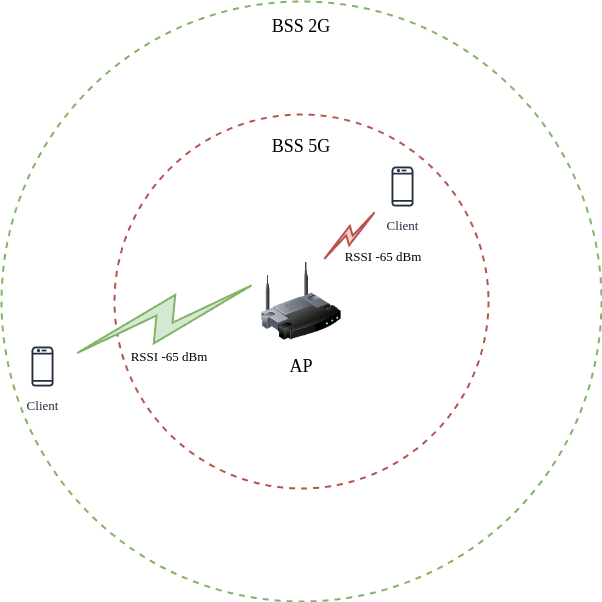
\includegraphics[width=0.75\textwidth]{mainmatter/images/BandSteering.png}
\caption{\label{fig:BandSteering} Mô hình chuyển băng tần}
\end{figure}

\subsubsection{ Chuyển vùng giữa các AP}
Chức năng này giúp hệ thống Mesh vượt trội hơn các hệ thống mở rộng vùng phủ Wi-Fi truyền thống khác. Các thiết bị kết nối trong mạng khi di chuyển giữa các vùng phủ của AP sẽ được tự động gợi ý chuyển vùng sang AP cho kết nối Wi-Fi tốt nhất so với vị trí của STA trong mạng. Bản tin đo và gợi ý cho STA lần lượt tuân theo chuẩn 802.11k và 802.11v, các thông số trên các bản tin này được thay đổi tùy thuộc vào cách nhà phát triển chức năng thiết kế.

\begin{figure}
\centering
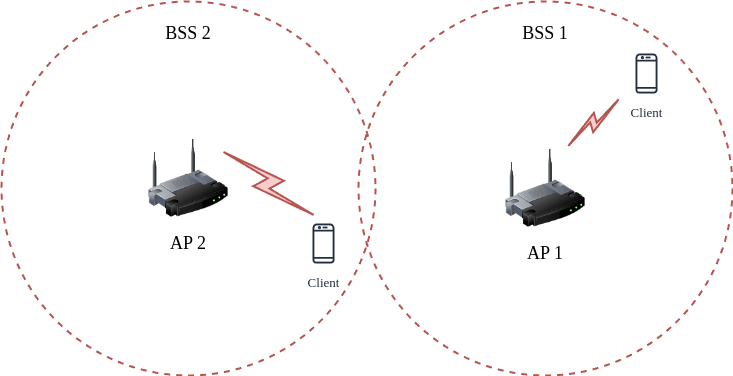
\includegraphics[width=1\textwidth]{mainmatter/images/Roaming.png}
\caption{\label{fig:topology} Mô hình chuyển vùng giữa các AP}
\end{figure}

\begin{table}[ht]
    \centering
    \caption{Nội dung bản tin AP Policy Request trong IEEE 1905.1 / EasyMesh}
    \begin{tabular}{|>{\raggedright\arraybackslash}m{5cm}|>{\raggedright\arraybackslash}m{8cm}|}
    \hline
    \textbf{TLV (Type-Length-Value)} & \textbf{Mô tả} \\
    \hline
    \textbf{AL MAC Address TLV} & Địa chỉ MAC lớp Abstraction Layer của thiết bị gửi bản tin. \\
    \hline
    \textbf{AP Radio Identifier TLV} & Xác định radio (băng tần) của AP mà policy được yêu cầu. \\
    \hline
    \textbf{AP Policy Request TLV} & Yêu cầu chính sách cấu hình AP, có thể chứa các tham số như băng tần ưu tiên, kênh, công suất phát... \\
    \hline
    \textbf{Vendor Specific TLV (tuỳ chọn)} & Thông tin mở rộng hoặc đặc thù theo nhà sản xuất. \\
    \hline
    \end{tabular}
\end{table}

\begin{table}[ht]
    \centering
    \caption{Nội dung bản tin Combined Infrastructure Metrics trong IEEE 1905.1 / EasyMesh}
    \begin{tabular}{|>{\raggedright\arraybackslash}m{5cm}|>{\raggedright\arraybackslash}m{8cm}|}
    \hline
    \textbf{TLV (Type-Length-Value)} & \textbf{Mô tả} \\
    \hline
    \textbf{AL MAC Address TLV} & Địa chỉ MAC lớp Abstraction Layer của thiết bị gửi bản tin (thường là Agent). \\
    \hline
    \textbf{Combined Infrastructure Metrics TLV} & TLV chính của bản tin. Tổng hợp các chỉ số hiệu năng liên kết backhaul giữa các thiết bị trong mạng mesh (có thể gồm Wi-Fi, Ethernet, MoCA, Powerline). \\
    \hline
    \textbf{Transmitter Link Metric TLV (tuỳ chọn)} & Nếu gửi chi tiết từng liên kết truyền – cung cấp thông tin throughput, RSSI, error rate,... \\
    \hline
    \textbf{Receiver Link Metric TLV (tuỳ chọn)} & Nếu gửi chi tiết từng liên kết nhận – tương tự thông tin hiệu năng đầu vào. \\
    \hline
    \textbf{Vendor Specific TLV (tuỳ chọn)} & Dữ liệu mở rộng riêng của nhà sản xuất (ví dụ thuật toán định tuyến nội bộ, chỉ số bổ sung,...). \\
    \hline
    \end{tabular}
\end{table}

\begin{table}[ht]
\centering
\caption{Nội dung bản tin Link Metric Query trong IEEE 1905.1}
\begin{tabular}{|>{\raggedright\arraybackslash}m{5cm}|>{\raggedright\arraybackslash}m{8cm}|}
\hline
\textbf{TLV (Type-Length-Value)} & \textbf{Mô tả} \\
\hline
\textbf{AL MAC Address TLV} & Địa chỉ MAC lớp Abstraction Layer của thiết bị gửi bản tin (thiết bị yêu cầu). \\
\hline
\textbf{Link Metric Query TLV} & TLV chính yêu cầu thông tin liên kết giữa thiết bị gửi và một hoặc nhiều thiết bị đích. Có thể chỉ định: \newline
- Địa chỉ MAC đích \newline
- Loại metric yêu cầu: Transmitter, Receiver hoặc cả hai. \\
\hline
\textbf{Vendor Specific TLV (tuỳ chọn)} & Dữ liệu mở rộng riêng của nhà sản xuất. \\
\hline
\end{tabular}
\end{table}

\begin{table}[ht]
\centering
\caption{Nội dung bản tin Link Metric Response trong IEEE 1905.1}
\begin{tabular}{|>{\raggedright\arraybackslash}m{5cm}|>{\raggedright\arraybackslash}m{8cm}|}
\hline
\textbf{TLV (Type-Length-Value)} & \textbf{Mô tả} \\
\hline
\textbf{AL MAC Address TLV} & Địa chỉ MAC lớp Abstraction Layer của thiết bị gửi bản tin (thiết bị phản hồi). \\
\hline
\textbf{Transmitter Link Metric TLV} & Chứa thông tin về hiệu năng liên kết truyền đi (Tx) từ thiết bị này đến các thiết bị lân cận. Bao gồm: \newline
- MAC đích \newline
- Throughput ước tính \newline
- RSSI \newline
- Phần trăm lỗi \\
\hline
\textbf{Receiver Link Metric TLV} & Chứa thông tin về hiệu năng liên kết nhận về (Rx) từ các thiết bị khác. Bao gồm các chỉ số tương tự như trên. \\
\hline
\textbf{Vendor Specific TLV (tuỳ chọn)} & Dữ liệu mở rộng riêng của nhà sản xuất (ví dụ: chỉ số độ trễ, jitter, hoặc số liệu nâng cao khác). \\
\hline
\end{tabular}
\end{table}

\begin{table}[ht]
\centering
\caption{Nội dung bản tin AP Link Metric Query trong IEEE 1905.1 / EasyMesh}
\begin{tabular}{|>{\raggedright\arraybackslash}m{5cm}|>{\raggedright\arraybackslash}m{8cm}|}
\hline
\textbf{TLV (Type-Length-Value)} & \textbf{Mô tả} \\
\hline
\textbf{AL MAC Address TLV} & Địa chỉ MAC lớp Abstraction Layer của thiết bị gửi bản tin (Controller). \\
\hline
\textbf{AP Metrics Query TLV} & TLV chính của bản tin. Cho biết Controller đang yêu cầu dữ liệu hiệu năng của một hoặc nhiều BSS/Radio thuộc AP. \newline
Có thể chứa: \newline
- MAC địa chỉ của AP Agent \newline
- BSSID cụ thể (nếu yêu cầu chi tiết) \newline
- Loại metric cần thu thập. \\
\hline
\textbf{Vendor Specific TLV (tuỳ chọn)} & Trường mở rộng để yêu cầu thêm chỉ số đặc thù của nhà sản xuất hoặc giải pháp cụ thể. \\
\hline
\end{tabular}
\end{table}

\begin{table}[ht]
\centering
\caption{Nội dung bản tin AP Link Metric Response trong IEEE 1905.1 / EasyMesh}
\begin{tabular}{|>{\raggedright\arraybackslash}m{5cm}|>{\raggedright\arraybackslash}m{8cm}|}
\hline
\textbf{TLV (Type-Length-Value)} & \textbf{Mô tả} \\
\hline
\textbf{AL MAC Address TLV} & Địa chỉ MAC lớp Abstraction Layer của thiết bị gửi bản tin (Agent). \\
\hline
\textbf{AP Metrics Response TLV} & TLV chính chứa các chỉ số hiệu năng về liên kết giữa các AP. Bao gồm: \newline
- BSSID hoặc Radio MAC \newline
- Chỉ số traffic (uplink/downlink) \newline
- Channel utilization (mức sử dụng kênh) \newline
- Error rate (tỉ lệ lỗi) \newline
- Retransmission count, và các chỉ số hiệu suất khác. \\
\hline
\textbf{Vendor Specific TLV (tuỳ chọn)} & Trường mở rộng chứa các chỉ số bổ sung theo nhà sản xuất (ví dụ như SNR, latency, jitter,...). \\
\hline
\end{tabular}
\end{table}

\section{Một số vấn đề trong mạng Wi-Fi Mesh cần lưu ý}
Ta thấy rằng các BSS trên các AP được chia làm 3 loại rất rõ ràng gồm fBSS, bBSS, bSTA. Trong quá trình phát triển hệ thống Mesh ta cần chú ý thực hiện cấu hình vai trò BSS này chính xác xuống Driver Wi-Fi, một số lỗi sẽ phát sinh khi ta không cấu hình đúng các BSS này. 

Bên cạnh đó, việc kết nối giữa các cặp Controller và Agent được thực hiện ban đầu đều là một-một, điều này thật là đơn giản nhưng vấn đề xuất hiện khi bạn thực hiện khởi động lại nguồn hoặc yêu cầu các Agent kết nối lại đến Controller. Việc này diễn ra khi các Agent kết nối vật lý (Wi-Fi hoặc Ethernet) thành công tới Controller và quá trình gửi bản tin đồng bộ giữa các AP sẽ phát sinh vấn đề khi thuật toán đồng bộ giữa các AP có sự khác biệt. Ta sẽ gặp vấn đề này khi thực hiện kết nối giữa các AP phiên bản khác nhau và bạn cần lưu ý để tránh gặp trường hợp không đồng bộ được cấu hình từ Controller tới các Agent.

Không chỉ dừng lại ở đó, các thuật toán chuyển vùng giữa các AP khác phiên bản đôi khi sẽ có những sự khác biệt, bản sau sẽ có thuật toán tốt hơn bản trước nhưng bản trước thì đã triển khai lượng lớn thiết bị dưới thị trường và bạn chưa thể cập nhật phần mềm cho tất cả chúng. Bạn cần chú ý cả vai trò Controller khi các phiên bản khác nhau đảm nhận vai trò này sẽ dẫn tới thuật toán chuyển vùng sẽ không hoạt động như mong muốn và bạn cần sửa đổi thuật toán khi phát hiện ra vấn đề này.

Điều cuối cùng cần quan tâm là phần cứng hay nói gần hơn là driver của Wi-Fi và Switch. Hai thứ này hoạt động đúng và ổn định theo thiết kế thì mới đảm bảo hệ thống Wi-Fi Mesh của bạn hoạt động tốt được. Một vài lỗi sẽ phát sinh từ đây và bạn cần lưu ý và nghiên cứu cả chúng để có thể phát triển hệ thống mạng Wi-Fi Mesh.